\chapter{Uživatelské testování}

\section{System Usability Scale (SUS)}
System Usability Scale\footnote{\url{https://www.usability.gov/how-to-and-tools/methods/system-usability-scale.html}\nocite{SystemUsabilityScaleSUSUsabilitygov-2020-06-16}} je jednoduchý test na přívětivost uživatelského rozhraní aplikace. Cílem tohoto testování je seznámit uživatele s aplikací a pak mu položit 10 otázek, které SUS definuje. Na základě odpovědí na tyto otázky je pak spočteno skóre uživatelské přívětivosti. Aby testování bylo objektivní, je potřeba aplikaci testovat na osobách, jež se nepodílely na žádné části softwarového vývoje.

Testovaným osobám bude vysvětlen základní princip fungování aplikace a poté jim budou určeny jednoduché úkoly, které musí splnit. Znění těchto úkolů bude úmyslně napsáno velmi obecně a nebudou použity termíny, jež jsou použity v aplikaci. Testovaná osoba pak musí sama přijít na to, jak danou akci provést a díky tomu bude schopna objektivně zhodnotit přívětivost uživatelského rozhraní.

\begin{enumerate}
    \item Zjistěte, které taxony řadíme pod Vyšší rostliny (latinsky Embryophyta).
    \item Pokuste se vyrobit graf podobný grafu na obrázku. Toto uspořádání vrcholů do stromu se nazývá \textbf{dagre}. Konkrétní pořadí vrcholů není důležité. Místo ručního hledání Pteropsidy a moss se je pokuste vyhledat pomocí jejich názvu.
    \begin{figure}[h]
        \centering
        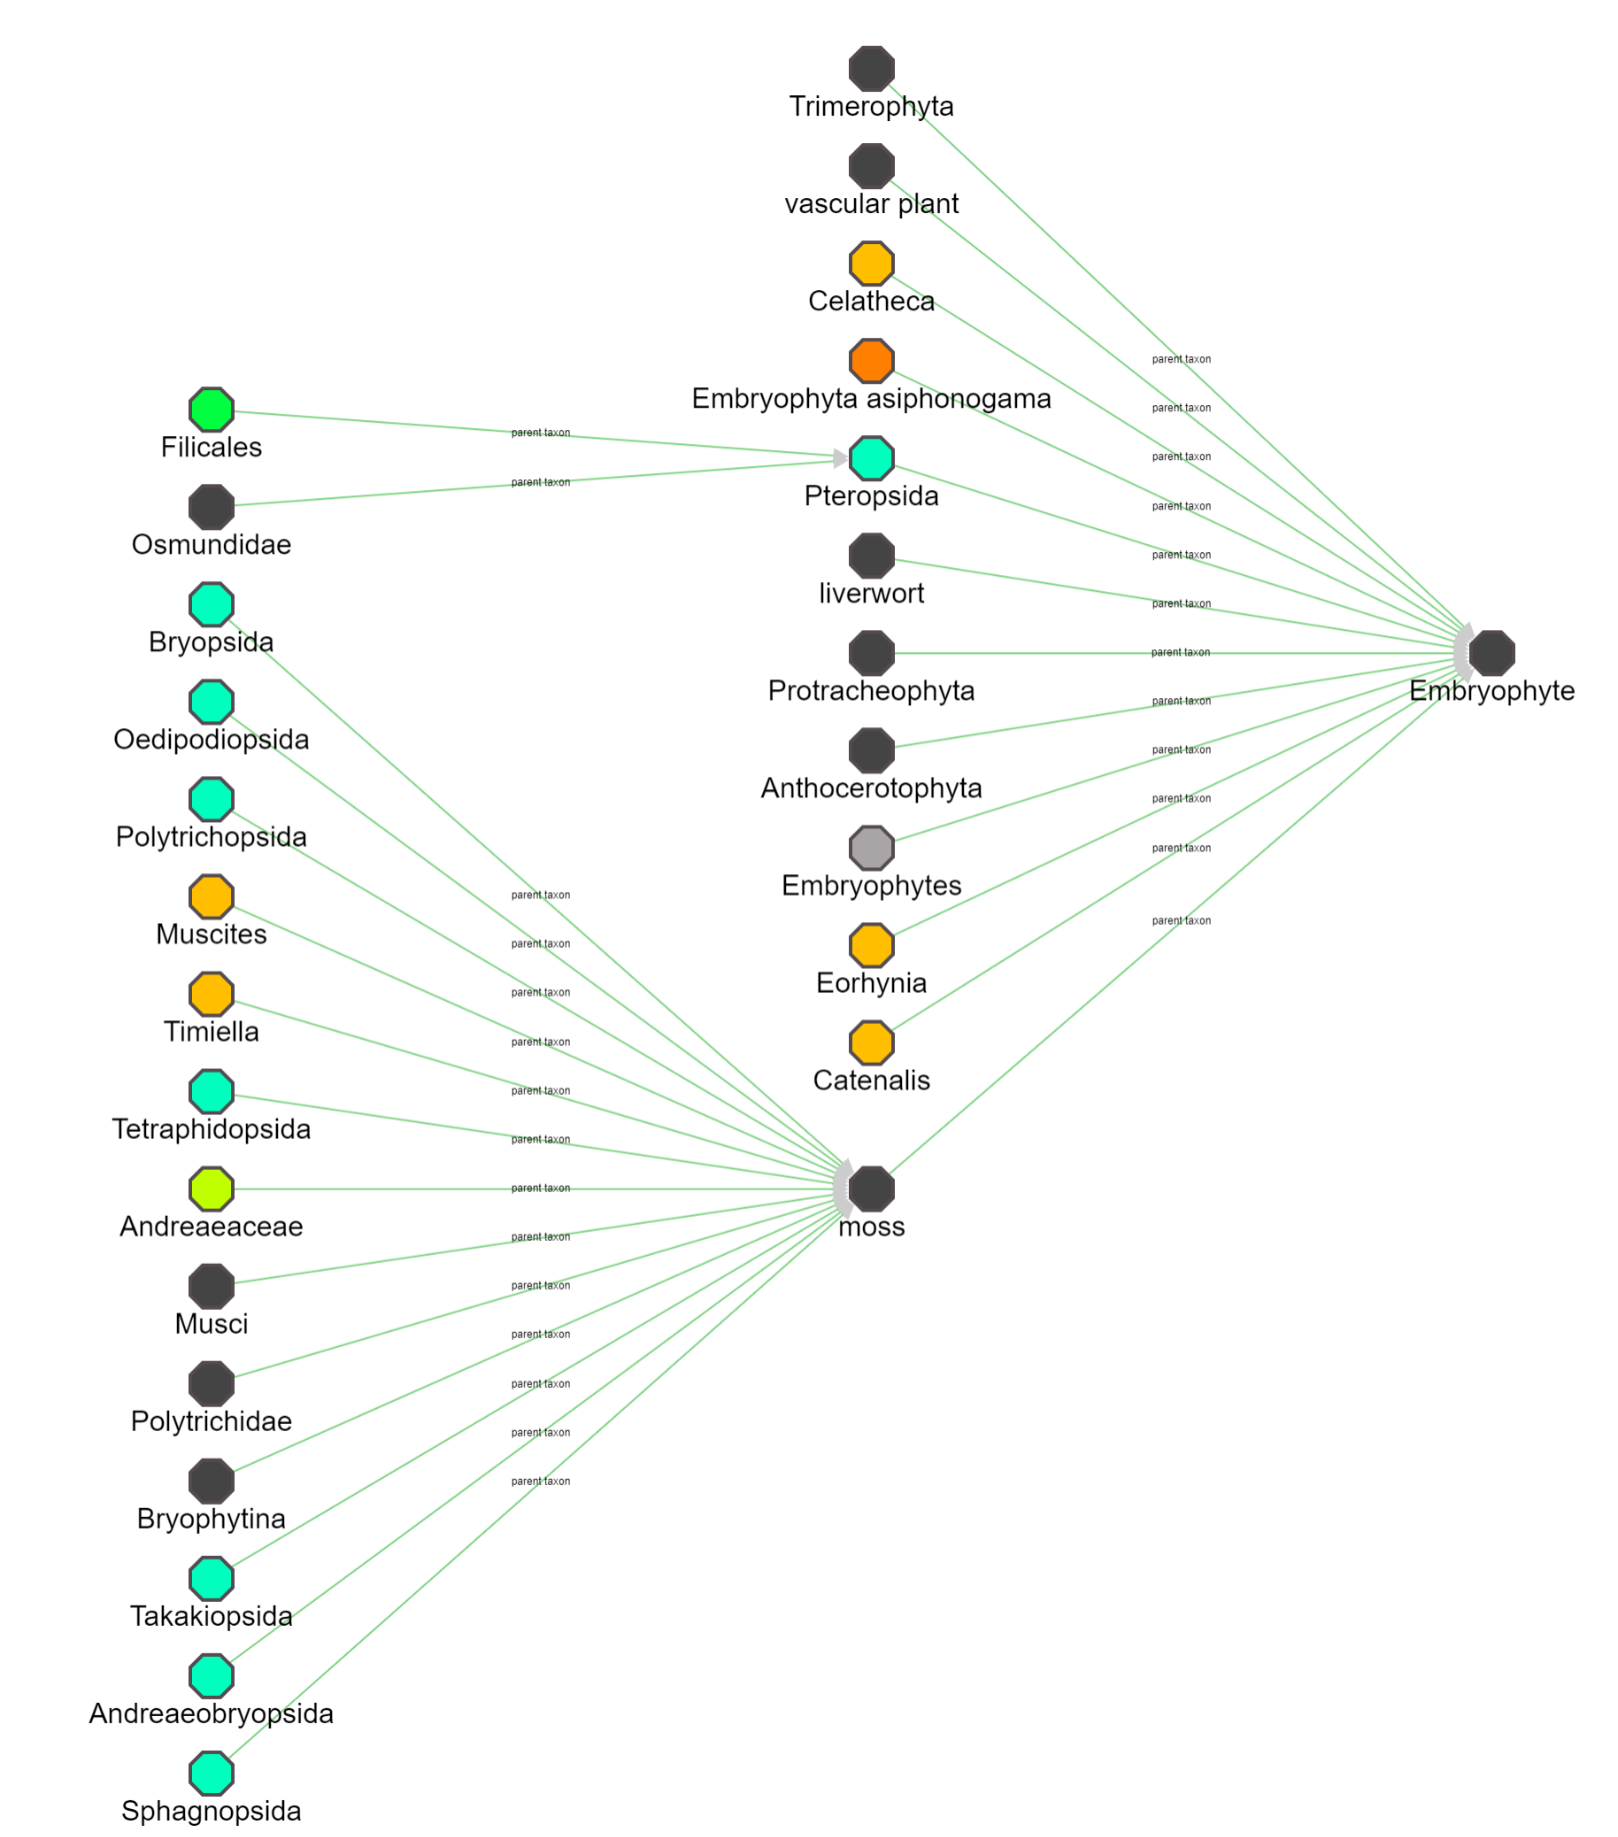
\includegraphics[width=0.5\textwidth]{media/sus-dagre.png}
    \end{figure}
    \item Stáhněte si aktuální graf do souboru, stránku aktualizujte a graf ze souboru opět načtěte.
    \item Nechte si zobrazit ze všech vrcholů jen ty, co mají třídu \uv{genus} (tedy chceme ty taxony, jež reprezentují rod).
    \item Odstraňte z grafu libovolný vrchol.
\end{enumerate}

\subsection{Výsledky testování SUS}

Na testování se podílelo celkem 13 respondentů. Níže je vypsán seznam deseti SUS otázek společně s výsledky testu.

\pgfplotstableread[row sep=\\,col sep=&]{
    score & count \\
    1 & 0 \\
    2 & 1 \\
    3 & 3 \\
    4 & 6 \\
    5 & 3 \\
}\dataone

\begin{tikzpicture}
    \begin{axis}[
            ybar,
            symbolic x coords={1,2,3,4,5},
            xtick=data,
        ]
        \addplot table[x=score,y=count]{\dataone};
    \end{axis}
\end{tikzpicture}

\section{Výsledky obecných otázek}
V rámci testování SUS byli respondenti navíc dotázáni, jaké části aplikace pro ně byly uživatelsky nepřívětivé a čemu neporozuměli. Výsledky jsou sepsány v následujícím seznamu.

\begin{itemize}
    \item Tlačítka v pravém dolním rohu grafové oblasti sloužící na obsluhu grafu (layoutování, zobrazení celého grafu, kompaktní mód) nejsou popsány a respondent odpověděl, že měl problém zjistit, co dělají.

    Tlačítkům bude vhodné přidat tooltipy vysvětlující jejich funkce obdobně, jak je tomu v jiných částech aplikace.
    \item Respondent nepochopil uživatelské rozhraní pro výběr layoutu. Neuvědomil si, že jednotlivé karty odpovídají konkrétním layoutům a vždy je aktivní pouze jeden layout. Měnil nastavení jiného layoutu, než toho, který byl aktivní.

    Zvážit kompletní změnu uživatelského rozhraní, které uživatele nutí nejprve zvolit layout a poté měnit jeho natavení.
\end{itemize}

\bigskip

Úkoly popsané v rámci SUS průzkumu sloužily také jako určitá forma uživatelského testování aplikace. I když nebylo jasně definováno, jak by aplikace měla na konkrétní úkoly reagovat, můžeme předpokládat, že úkoly proběhly úspěšně, neboť je všichni z respondentů dokončili. Měřením code coverage bylo zjištěno, že provedením všech úkolů bylo pokryto 77\% kódu. Většina aplikace tedy byla těmito úkoly úspěšně otestována. \uv{Provedením úkolů} je myšlena nejjednodušší cesta, jak lze daný úkol v aplikaci provést.

Měření bylo prováděno s pomocí IDE WebStorm\footnote{\url{https://www.jetbrains.com/webstorm/}} od JetBrains pod prohlížečem Google Chrome. Code coverage se měří z řádků, které byly v aplikace spuštěny, přičemž se do výpočtu podílu nezahrnují komentáře, prázdné řádky a definice rozhraní, které se do JavaScriptu nepřekládají.